
\subsection{Model Setup}
\subsubsection{Model Domain}
The domain of the model is bounded by longitudes $\phi_E=-180^{\circ}$ and $\phi_W=-180^{\circ}$ and latitudes $\theta_N=80^{\circ}$ and $\theta_S=-80^{\circ}$ with periodic boundary conditions in the zonal direction.
Furthermore the model uses restoring boundary conditions. Restoring the boundary at the surface of the oceanic basin to be a value based of a forcing field for Sea Surface Temperature (SST), Sea Surface Salinity (SSS), wind stresses ($\tau$) and heat flux.
 The depth profile has 15 layers with grid stretching (\fref{fig:gridstrech}). There are $90 \times 40$ grid points to make a $4^{\circ} \times 4^{\circ}$ resolution model.
 
 \begin{figure}[H]
 	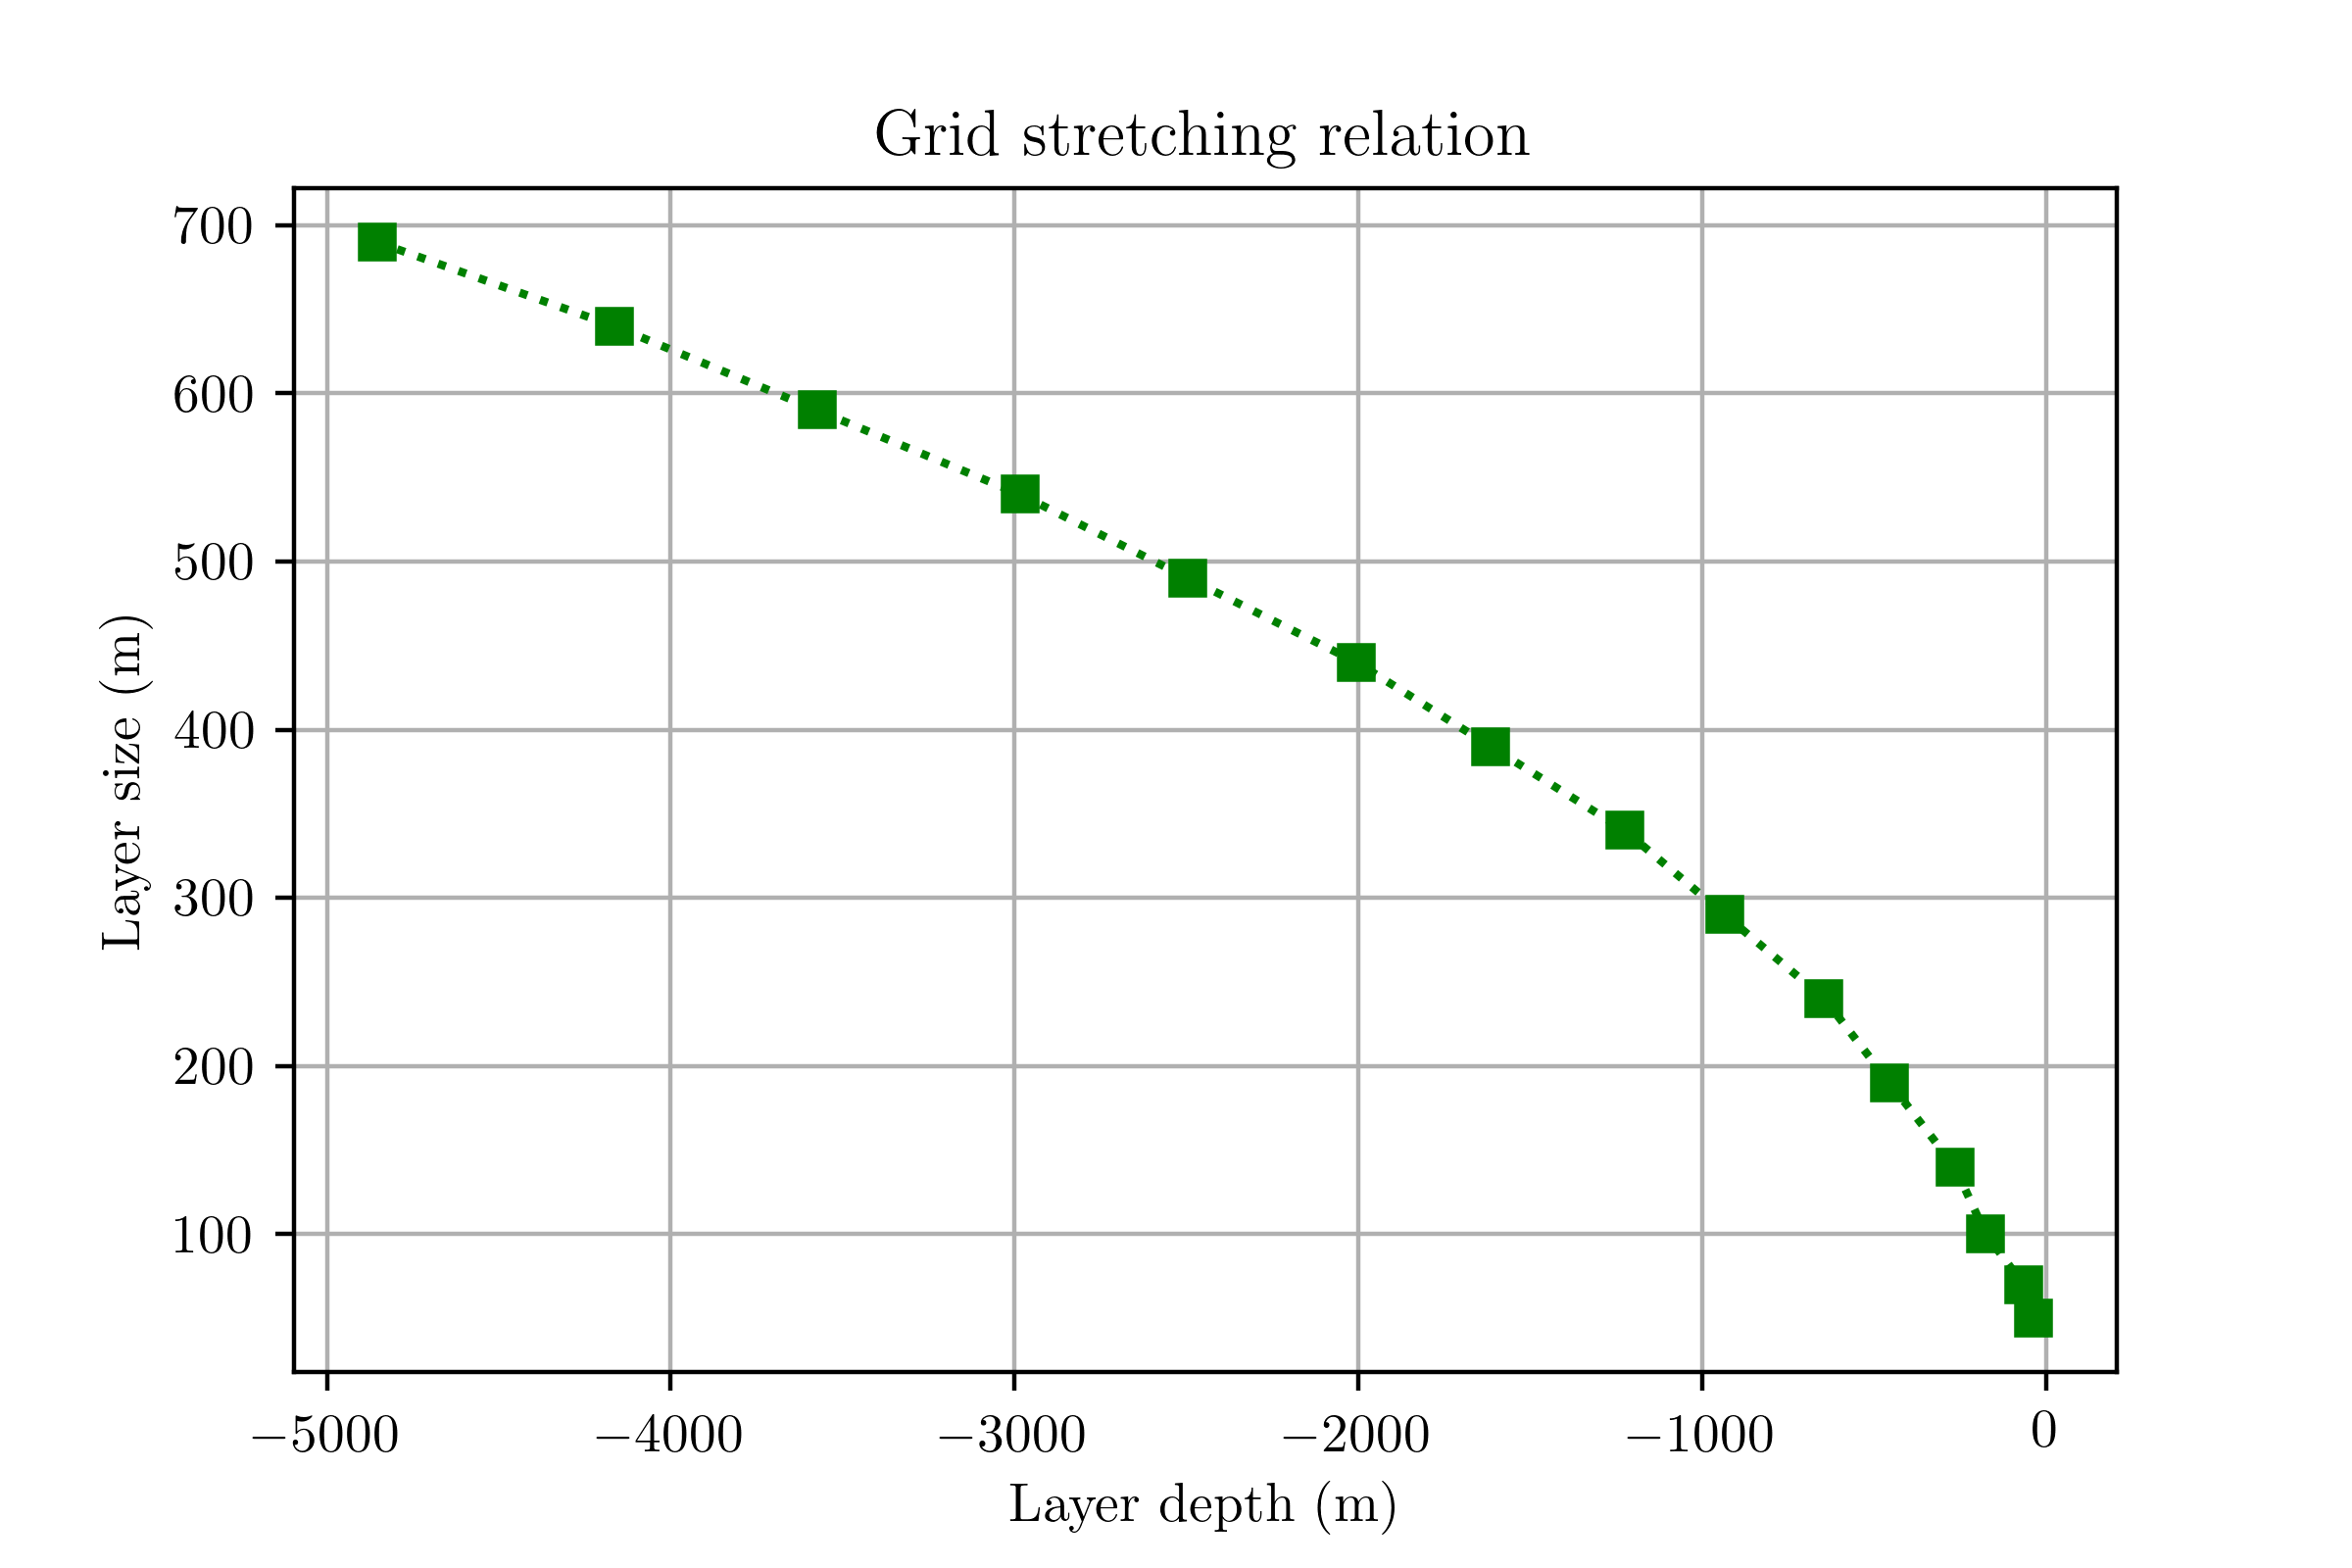
\includegraphics[width=\linewidth]{grid_stretching.png}
 	\caption{Grid stretching relation used}
 	\label{fig:gridstrech}
 \end{figure}

\subsubsection{Surface Forcings}
 Choosing the correct forcing for the ocean is very important. It is known that in general circulation models the MOC is highly sensitive too even small changes in surface forcings (\cite{Milliff1999May}). Attempts at making these forcings highly idealized have often been made in the past with varying rates of success. In this paper we will however use idealized forcings. Noting the fact that, this will probably induce the aforementioned errors in deep ocean circulations.
 
 There were several methods that are explored when it comes to creating these idealized forcings. In the \cite{Mulder2017Jul} paper an analytic forcing profile was used for wind flux, SST and SSS. This however fails to capture seasonal changes in each of the forcings due to the earths axial tilt. Something that can bring about a huge effect on the strength of the MOC. To combat this change a compromise is proposed. The SSS, SST and heat flux profiles are taken as zonal means for each month in the earths rotation. While the Zonal wind stress is set to the simple profile proposed by \cite{bryan1987parameter}. The analytic wind stress profile used in the paper is not specified specifically. However, it can quite easily be deduced from the profile's plot. The choice of this analytic profile was made over a zonally averaged and equatorial averaged forcing $\mu(\tau_x)$. These were both tested on the present day configuration to see which of these forcings most accurately captures the present day MOC. In \fref{sec:MOCSTREAM} a comparison with the present day MOC and BSF is made. 
 
 \subsubsection{Forcing errors}
 (TODO)
 \subsubsection{Initial conditions}
 (TODO)
 
 \subsubsection{MOC stream function} \label{sec:MOCSTREAM}
 
 The global Meridional Overturning Circulation $\Psi_{MOC}$ is defined as the zonally integrated meridional volume transport of water in the worlds oceans. It can be written down as:
 
 $$
 \Psi_{MOC}(y,z) = \int_{z}^{0} \int_{-180^{\circ}}^{180^{\circ}} v(x,y,z') dx dz'
 $$
Where $v$ is the meridional component of the velocity.
$ \Psi_{MOC}$ is thus a stream function of the zonally integrated volume transport in the Earth's water basins. Plotting this stream function can give a lot of insight into the deep water transport associated with the thermohaline circulation. In this paper we hope to capture these deep water transport formations.

(Image showing the regions and their names)

\subsubsection{Barotropic Stream Function} \label{sec:BSF_theory}
It it furthermore interesting to look at an expression for the transport of ocean gyres. We know that the depth integrated flow must be horizontally non-divergent. Thus a streamfunction $\Psi_{b}$ can be introduced. Where $v(x,y,z)$ is the meridional velocity:
\begin{align}
U = -\frac{\partial \Psi_{b}}{\partial y}; V=\frac{\partial \Psi_{b}}{\partial x} \\
\Psi_{b} = \int_{eastern bdy}^{x} \int_{-D}^{0} v(x',y,z) dz dx'
\end{align}

Thus this so called barotropic stream function $\Psi_{b}$ is defined by integrating the meridional transport westward from the eastern boundary of the domain. It is a useful tool to look at the shape and gyres associated with the major ocean current systems. By using the Sverdrup relation
$$
\int_{-D}^{0}v(x,y,z) dz = \frac{1}{\beta \rho_{ref}}\vec{\hat{z}}\cdot \nabla \times \tau
$$

 first proposed by \cite{sverdrup1947wind} we can look at a schematic diagram of the barotropic stream function based on the prevailing zonal winds. \fref{fig:schem_currents} shows a schematic of this relation. It is easily visible how the prevailing zonal winds relate to the wind stress forcing seen in \fref{fig:idealized_forc}. The calculation of the barotropic streamfunction without easily defined boundaries, is quite a complicated process done by Veros. 
 
 
 (probably will add a discussion on this)
 
  \begin{figure}[H]
 	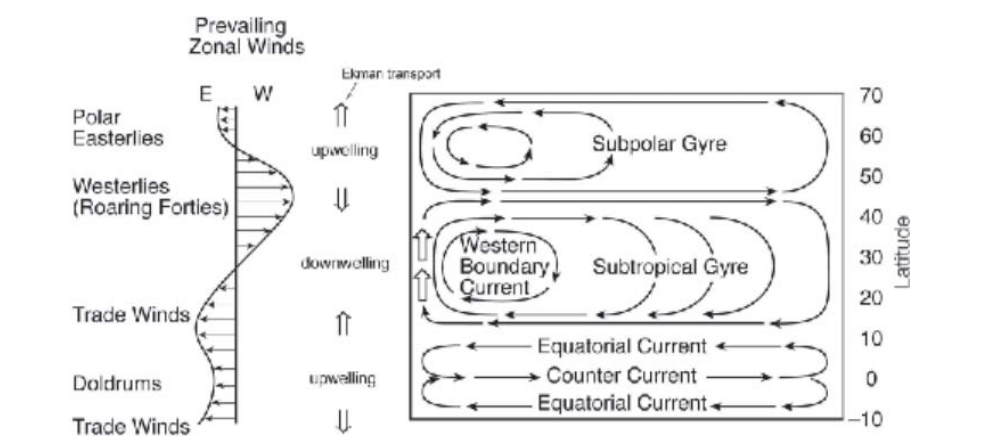
\includegraphics[width=\linewidth]{schematic_marshall_plumb.png}
 	\caption{Schematic of the barotropic stream function based on the Sverdrup relation. Showing the subpolar and subtropical Gyres and equatorial currents. Figure taken from \cite{MarschallPlumb}}
 	\label{fig:schem_currents}
 \end{figure}
\subsubsection{Passage throughflow}\label{sec:throughflowp}
For each of the passages mentioned in \fref{sec:bathys} it is interesting to talk about the total volume transport through each of the passages discussed in \fref{sec:bathys}. This is done using a simple integration to calculate the volumetric flux through each passage. This volumetric flux, defined as

\begin{align}
Q = \iint_A \vec{u} \cdot d\vec{A}
\end{align}	

For each passage a suitable location is chosen such that there are no boundaries next to the passageways, this is done for each time step. Then the $u$ component of the flow is used to compute the total flow. This method is the same for each of the passages and thus we can study the effect of changes in bathymetry to on the relative strength of the flow. However, it should be noted that these values may not represent real physical values. As the passages in a $4^{\circ}$ model are often only a few grid cells wide. Resulting in discrepancies in the calculation of the throughflow due to boundary conditions. 
There is however a more accurate way to calculate these throughflows. This can be done using the output of the Barotropic stream function discussed in \fref{sec:BSF_theory}. This also gives us a measure of (purely zonal) throughflow in each grid cell. It is however difficult to get accurate values from this in Veros because the current version does not display the boundary values for the stream function.

